\section{Von Handwerk zu Engineering: Die BEATRIX-Transformation}
%==============================================================================

\epigraph{\textit{``Software engineering is what happens to programming when you add time and other programmers.''}}{--- Russ Cox}

Die bisherigen Abschnitte haben die axiomatischen Grundlagen des BCM und die technischen Komponenten von BEATRIX beschrieben. Dieser Abschnitt adressiert eine fundamentale Frage: \textbf{Warum war eine systematische, skalierbare Verhaltensparameter-Schätzung vor LLMs nicht möglich?}

Die Antwort liegt in der Struktur des klassischen BCM-Prozesses, der als \textit{fragmentiertes Handwerk} charakterisiert werden kann -- im Gegensatz zum \textit{integrierten Engineering-Prozess}, den BEATRIX ermöglicht.

\subsection{Der Pre-LLM BCM-Prozess: Fragmentiertes Handwerk}

\subsubsection{Die fragmentierte Wertschöpfungskette}

Der klassische Prozess der Verhaltensparameter-Schätzung besteht aus vier Schritten mit systematischen Bruchstellen:

\begin{figure}[h]
\centering
\begin{tikzpicture}[
    node distance=0.8cm,
    step/.style={rectangle, draw, rounded corners, minimum width=2.2cm, minimum height=1.2cm, align=center, font=\small},
    break/.style={draw=red!70, dashed, thick},
    arrow/.style={->, thick, >=stealth}
]

% Steps
\node[step, fill=blue!10] (s1) at (0, 0) {Kontext\\verstehen};
\node[step, fill=blue!10] (s2) at (3.5, 0) {Verhaltens-\\annahmen\\bilden};
\node[step, fill=blue!10] (s3) at (7, 0) {Parameter-\\schätzung};
\node[step, fill=blue!10] (s4) at (10.5, 0) {BCM-\\Modellierung};

% Arrows with breaks
\draw[arrow] (s1) -- node[above, font=\scriptsize, red!70] {Bruch 1} (s2);
\draw[arrow] (s2) -- node[above, font=\scriptsize, red!70] {Bruch 2} (s3);
\draw[arrow] (s3) -- node[above, font=\scriptsize, red!70] {Bruch 3} (s4);

% Outputs below
\node[below=0.5cm of s1, font=\scriptsize, text=gray] {Dokument};
\node[below=0.5cm of s2, font=\scriptsize, text=gray] {Kopf des\\Beraters};
\node[below=0.5cm of s3, font=\scriptsize, text=gray] {Notiz\\(vielleicht)};
\node[below=0.5cm of s4, font=\scriptsize, text=gray] {Excel/\\Python};

% Missing feedback
\node[below=1.8cm of s2, font=\scriptsize, red!70] {Bruch 4: Kein Feedback-Loop};
\draw[break, <->] (0, -1.8) -- (10.5, -1.8);

\end{tikzpicture}
\caption{Die fragmentierte Wertschöpfungskette des Pre-LLM BCM-Prozesses mit vier systematischen Bruchstellen.}
\label{fig:fragmented-chain}
\end{figure}

\paragraph{Die Handwerk-Probleme im Überblick.}
\begin{itemize}
    \item \textbf{Nicht reproduzierbar}: Jeder Berater macht es anders
    \item \textbf{Nicht skalierbar}: Linear mit Beraterkapazität
    \item \textbf{Qualitätsvariation}: Abhängig von Tagesform, Erfahrung, Zeitdruck
    \item \textbf{Wissenserosion}: Wissen bleibt in Köpfen, nicht im System
    \item \textbf{Keine Lernschleife}: Fehler werden nicht systematisch erfasst
\end{itemize}

\subsubsection{Bruch 1: Kontext → Verhaltensannahmen}

\paragraph{Das Problem: Informationsverlust.}
Ein typischer 2-Stunden-Workshop mit Stakeholdern produziert 50+ verhaltensrelevante Aussagen:

\begin{quote}
\textit{``Unsere Kunden sind sehr preisbewusst''} \\
\textit{``Die älteren Kunden sind loyaler''} \\
\textit{``Im B2B-Segment entscheiden Einkäufer rational''} \\
\textit{``Qualität ist wichtiger als Preis''} (Widerspruch zu Aussage 1!) \\
... und 46 weitere Aussagen ...
\end{quote}

\paragraph{Was der Berater mitnimmt:}
\begin{itemize}
    \item Die 3--4 Aussagen, die er sich gemerkt hat
    \item Gefiltert durch seine eigenen kognitiven Biases
    \item Ohne Gewichtung nach Evidenzstärke
    \item Ohne Dokumentation der Widersprüche
\end{itemize}

\textbf{Geschätzter Informationsverlust}: $\approx 80\%$

\subsubsection{Bruch 2: Verhaltensannahmen → Parameter}

\paragraph{Das Problem: Willkürliche Übersetzung.}

Der Berater denkt: \textit{``Die Kunden sind preisbewusst.''}

Was bedeutet das für BCM-Parameter?

\begin{table}[h]
\centering
\caption{Willkürliche Parameter-Übersetzung im klassischen Prozess}
\small
\begin{tabular}{@{}lll@{}}
\toprule
\textbf{Parameter} & \textbf{Berater-Überlegung} & \textbf{Basis} \\
\midrule
$\lambda$ (Loss Aversion) & ``Höher als normal? Vielleicht 2.5?'' & Intuition \\
Reference Point & ``Was ist der Referenzpreis? Keine Ahnung.'' & Ignoriert \\
$w_F$ (Financial) & ``Financial wichtig... 0.4?'' & Aus der Luft \\
Elastizität & ``Keine Daten, ich nehme $-1.5$'' & ``Branchenstandard'' \\
\bottomrule
\end{tabular}
\end{table}

\textbf{Kernprobleme}:
\begin{itemize}
    \item Keine systematische Übersetzungslogik
    \item Keine Dokumentation der Reasoning-Kette
    \item Keine Base Rates als empirischer Anker
\end{itemize}

\subsubsection{Bruch 3: Parameter → Modell}

\paragraph{Das Problem: Händische Übertragung.}

Der Berater hat (irgendwo) notiert: \textit{``$\lambda \approx 2.5$, preissensitiv, ältere loyaler''}

Der Analyst muss ins Excel/Python-Modell übertragen:

\begin{verbatim}
lambda = 2.5   # TODO: check with PM
beta = 0.7     # default
alpha = ???    # was ist das?
\end{verbatim}

\textbf{Kernprobleme}:
\begin{itemize}
    \item Übertragungsfehler (Tippfehler, Verwechslungen)
    \item Unvollständige Spezifikation (fehlende Parameter)
    \item Keine Validierung (inkonsistente Werte möglich)
    \item Kontextverlust (``warum 2.5?'' nicht dokumentiert)
\end{itemize}

\subsubsection{Bruch 4: Kein Feedback-Loop}

\paragraph{Das Problem: Kein organisationales Lernen.}

\begin{quote}
\textbf{Modell-Output} (Januar): ``Bei 5\% Preiserhöhung $\rightarrow$ 3\% Churn'' \\
\textbf{Tatsächlicher Outcome} (Juli): 7\% Churn
\end{quote}

Was passiert typischerweise?

\begin{table}[h]
\centering
\caption{Typische Reaktionen auf Prognose-Fehler}
\begin{tabular}{@{}ll@{}}
\toprule
\textbf{Option} & \textbf{Konsequenz} \\
\midrule
A: Niemand vergleicht & ``Das Projekt ist abgeschlossen'' \\
B: Jemand merkt es & ``Das lag an externen Faktoren'' (keine Analyse) \\
C: Erkenntnis geht verloren & Berater nicht mehr im Projekt, Excel weg \\
D: Nächstes Projekt & ``Wir machen wieder einen Workshop...'' \\
\bottomrule
\end{tabular}
\end{table}

\textbf{Ergebnis}: \textbf{Kein organisationales Lernen}. Jedes Projekt startet bei Null.

\subsection{Die Analogie: Software 1980er vs. 2020er}

Die Transformation von BCM-Handwerk zu BEATRIX-Engineering entspricht der Evolution der Softwareentwicklung:

\begin{table}[h]
\centering
\caption{Analogie: Softwareentwicklung und BCM-Prozess}
\begin{tabular}{@{}p{5.5cm}p{5.5cm}@{}}
\toprule
\textbf{Software 1980er (Handwerk)} & \textbf{Software 2020er (Engineering)} \\
\midrule
Code auf Papier & Git Repository \\
Mündliche Übergabe & CI/CD Pipeline \\
``Funktioniert auf meinem Rechner'' & Docker Container \\
Keine Tests & Unit Tests, Integration Tests \\
Keine Dokumentation & Auto-generierte Docs \\
Wissen in Köpfen & Knowledge Base, Wiki \\
\bottomrule
\end{tabular}
\end{table}

\textbf{BCM heute = Software 1980er}:
\begin{itemize}
    \item Parameter in Köpfen / Notizen
    \item Mündliche Übergabe zwischen Berater und Analyst
    \item ``Funktioniert für diesen Kunden''
    \item Keine systematische Dokumentation
    \item Wissen geht mit Mitarbeitern
\end{itemize}

\subsection{Die Blockade: Warum war End-to-End nicht möglich?}

\subsubsection{Das Schwarze Loch: Natürliche Sprache → Parameter}

Der kritische Engpass lag in der Übersetzung von unstrukturiertem Text zu strukturierten Parametern:

\begin{figure}[h]
\centering
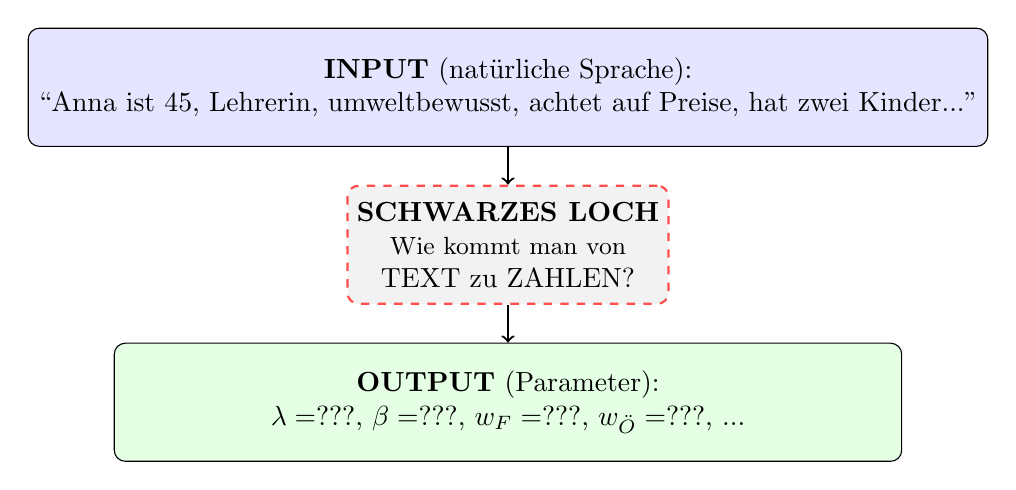
\begin{tikzpicture}[
    node distance=1.5cm
]

% Input
\node[rectangle, draw, rounded corners, fill=blue!10, minimum width=10cm, minimum height=1.5cm, align=center] (input) at (0, 2) {
    \textbf{INPUT} (natürliche Sprache):\\
    ``Anna ist 45, Lehrerin, umweltbewusst, achtet auf Preise, hat zwei Kinder...''
};

% Black hole
\node[rectangle, draw=red!70, dashed, thick, rounded corners, minimum width=4cm, minimum height=1.5cm, align=center, fill=gray!10] (hole) at (0, 0) {
    \textbf{SCHWARZES LOCH}\\
    \small Wie kommt man von\\
    TEXT zu ZAHLEN?
};

% Output
\node[rectangle, draw, rounded corners, fill=green!10, minimum width=10cm, minimum height=1.5cm, align=center] (output) at (0, -2) {
    \textbf{OUTPUT} (Parameter):\\
    $\lambda = ???$, $\beta = ???$, $w_F = ???$, $w_{\ddot{O}} = ???$, ...
};

% Arrows
\draw[->, thick] (input) -- (hole);
\draw[->, thick] (hole) -- (output);

\end{tikzpicture}
\caption{Das ``Schwarze Loch'' der Parameter-Schätzung: Der Übergang von natürlicher Sprache zu quantifizierten Parametern war der kritische Engpass.}
\label{fig:black-hole}
\end{figure}

\subsubsection{Pre-LLM Optionen -- und warum sie scheiterten}

\paragraph{Option 1: Mensch (Berater).}
\begin{itemize}
    \item[$-$] Langsam: 30--60 Minuten pro Persona
    \item[$-$] Teuer: Beraterhonorar (\EUR{50--200} pro Schätzung)
    \item[$-$] Inkonsistent: Verschiedene Berater $\rightarrow$ verschiedene Ergebnisse
    \item[$-$] Nicht dokumentiert: Reasoning im Kopf
    \item[$-$] Nicht skalierbar
\end{itemize}

\paragraph{Option 2: Regelbasiertes System.}
\begin{verbatim}
WENN Alter > 60 DANN lambda += 0.1
WENN "preisbewusst" IN text DANN w_F += 0.1
...
\end{verbatim}

\begin{itemize}
    \item[$-$] Kombinatorische Explosion: Tausende von Regeln nötig
    \item[$-$] Kontext wird ignoriert: ``preisbewusst'' bedeutet in verschiedenen Kontexten Verschiedenes
    \item[$-$] Neue Fälle nicht abgedeckt
    \item[$-$] Wurde versucht, hat nie skaliert
\end{itemize}

\paragraph{Option 3: Machine Learning (klassisch).}
Theoretisch möglich, aber:
\begin{itemize}
    \item[$-$] Bräuchte Labeled Training Data: Tausende Personas mit ``echten'' Parametern
    \item[$-$] \textbf{Diese Daten existieren nicht!}
    \item[$-$] Kein Transfer auf neue Domänen
    \item[$-$] Praktisch nicht umsetzbar
\end{itemize}

\textbf{Ergebnis}: Dieser Schritt blieb \textbf{manuelles Handwerk}.

\subsection{LLM als fehlende Brücke}

Large Language Models lösen das ``Schwarze Loch''-Problem durch eine einzigartige Kombination von Fähigkeiten:

\begin{figure}[h]
\centering
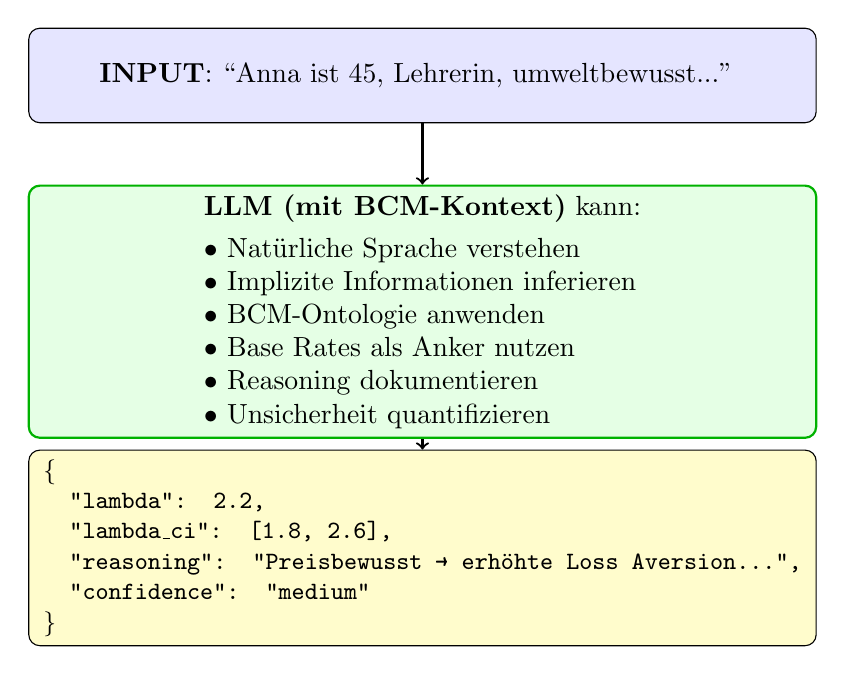
\begin{tikzpicture}[
    node distance=1.2cm
]

% Input
\node[rectangle, draw, rounded corners, fill=blue!10, minimum width=10cm, minimum height=1.2cm, align=center] (input) at (0, 3) {
    \textbf{INPUT}: ``Anna ist 45, Lehrerin, umweltbewusst...''
};

% LLM box
\node[rectangle, draw=green!70!black, thick, rounded corners, fill=green!10, minimum width=10cm, minimum height=3cm, align=left] (llm) at (0, 0) {
    \textbf{LLM (mit BCM-Kontext)} kann:\\[0.3em]
    $\bullet$ Natürliche Sprache verstehen\\
    $\bullet$ Implizite Informationen inferieren\\
    $\bullet$ BCM-Ontologie anwenden\\
    $\bullet$ Base Rates als Anker nutzen\\
    $\bullet$ Reasoning dokumentieren\\
    $\bullet$ Unsicherheit quantifizieren
};

% Output
\node[rectangle, draw, rounded corners, fill=yellow!20, minimum width=10cm, minimum height=2cm, align=left, font=\small\ttfamily] (output) at (0, -3) {
    \{\\
    \quad "lambda": 2.2,\\
    \quad "lambda\_ci": [1.8, 2.6],\\
    \quad "reasoning": "Preisbewusst → erhöhte Loss Aversion...",\\
    \quad "confidence": "medium"\\
    \}
};

% Arrows
\draw[->, thick] (input) -- (llm);
\draw[->, thick] (llm) -- (output);

\end{tikzpicture}
\caption{LLM als Brücke zwischen natürlicher Sprache und strukturierten BCM-Parametern.}
\label{fig:llm-bridge}
\end{figure}

\paragraph{Die kritischen Eigenschaften.}
\begin{enumerate}
    \item \textbf{Schnell}: Sekunden statt Stunden
    \item \textbf{Konsistent}: Gleicher Input $\rightarrow$ gleiches Output (bei fixierter Temperatur)
    \item \textbf{Dokumentiert}: Reasoning-Chain ist Teil des Outputs
    \item \textbf{Skalierbar}: 1000 Personas parallel möglich
    \item \textbf{Integrierbar}: API-basiert, kein Medienbruch
\end{enumerate}

\subsection{Die BEATRIX End-to-End Pipeline}

BEATRIX implementiert einen durchgängigen 6-Phasen-Prozess:

\subsubsection{Phase 1: Input Layer}

\begin{itemize}
    \item Akzeptiert verschiedene Formate: Workshop-Protokolle (.docx), CRM-Daten (.csv), Interview-Transkripte (.txt)
    \item BEATRIX Parser strukturiert unstrukturierten Input
    \item Keine manuelle Vorverarbeitung nötig
\end{itemize}

\subsubsection{Phase 2: Extraction Layer}

LLM extrahiert aus unstrukturiertem Input:
\begin{itemize}
    \item Demografische Merkmale
    \item Verhaltensrelevante Aussagen
    \item Kontextinformationen
    \item Widersprüche und Unsicherheiten
    \item Fehlende Informationen (Gaps)
\end{itemize}

\textbf{Output}: Strukturiertes Persona-Objekt

\subsubsection{Phase 3: Estimation Layer}

Die 4-Stufen-Architektur (vgl. Abschnitt~\ref{sec:4-stufen}) wird angewendet:

\begin{table}[h]
\centering
\caption{Parameter-Schätzung am Beispiel $\lambda$}
\begin{tabular}{@{}llr@{}}
\toprule
\textbf{Stufe} & \textbf{Quelle} & \textbf{$\lambda$-Beitrag} \\
\midrule
1: Base Rate & Gächter et al. & 2.00 \\
2: Demografie & Alter 45 & +0.10 \\
3a: Kontext (empirisch) & Low Stakes & $-0.10$ \\
3b: Kontext (LLM) & Umweltentscheidung & +0.15 \\
4: Persona (LLM) & ``preisbewusst'' & +0.05 \\
\midrule
\textbf{Final} & & \textbf{2.20} [1.7, 2.7] \\
\bottomrule
\end{tabular}
\\[0.3em]
\footnotesize Anteil empirisch: 81\%, Anteil LLM: 19\%
\end{table}

\textit{Wiederholen für alle Parameter: $\beta$, $\alpha$, $\beta_{FS}$, $w_F$, $w_E$, $w_P$, $w_S$, $w_D$, $w_{\ddot{O}}$, ...}

\subsubsection{Phase 4: Modeling Layer}

Parameter fließen \textbf{automatisch} in BCM-Modell:
\begin{itemize}
    \item Keine manuelle Übertragung
    \item Validierung gegen Constraints (z.B. $\beta_{FS} \leq \alpha$)
    \item Sensitivitätsanalyse automatisch
    \item Monte-Carlo für Unsicherheitspropagation
\end{itemize}

\subsubsection{Phase 5: Output \& Validation Layer}

Drei Output-Typen:
\begin{enumerate}
    \item \textbf{Prognose-Report}: ``Bei 5\% Preiserhöhung $\rightarrow$ 4\% Churn [2\%, 6\%]''
    \item \textbf{Audit-Trail}: Vollständige Dokumentation aller Schritte
    \item \textbf{Interventions-Empfehlung}: ``Framing auf Verlustvermeidung optimieren''
\end{enumerate}

\subsubsection{Phase 6: Feedback Layer}

Nach Implementierung:
\begin{itemize}
    \item Tatsächlicher Outcome wird erfasst
    \item Vergleich mit Prognose
    \item Optional: Bayesian Update der Base Rates
    \item Organisationales Lernen wird ermöglicht
\end{itemize}

\begin{quote}
\textit{``Prognose war 4\% Churn, tatsächlich 6\%''} \\
$\rightarrow$ \textit{``$\lambda$ war unterschätzt, Update: $\lambda_{prior} \mathrel{+}= 0.15$''}
\end{quote}

\subsection{Der Kontrast: Handwerk vs. Engineering}

\begin{table}[h]
\centering
\caption{Vergleich: Pre-LLM Handwerk vs. BEATRIX End-to-End}
\small
\begin{tabular}{@{}lcc@{}}
\toprule
\textbf{Dimension} & \textbf{Pre-LLM (Handwerk)} & \textbf{BEATRIX (E2E)} \\
\midrule
Medienbrüche & 3--4 pro Projekt & 0 \\
Dokumentation & Fragmentiert, oft fehlend & Automatisch, vollständig \\
Reproduzierbarkeit & Niedrig (personenabhängig) & Hoch (deterministisch) \\
Zeit pro Persona & 30--60 Minuten & 10--30 Sekunden \\
Skalierbarkeit & Linear mit Kapazität & Quasi-unbegrenzt \\
Konsistenz & Variiert & Garantiert \\
Wissenstransfer & Mündlich, informell & Systemisch, persistent \\
Lernfähigkeit & Ad-hoc, unsystematisch & Strukturiert, messbar \\
Audit-Fähigkeit & Schwierig bis unmöglich & Built-in \\
Kosten pro Schätzung & \EUR{50--200} & \EUR{0.01--0.10} \\
\bottomrule
\end{tabular}
\end{table}

\subsection{Das Axiom: MA-INF-08 End-to-End Integration}

Die Transformation von Handwerk zu Engineering wird im folgenden Axiom formalisiert:

\begin{axiom}[End-to-End Integration: MA-INF-08]
\begin{enumerate}
    \item BEATRIX implementiert einen \textbf{durchgängigen Prozess} von unstrukturiertem Input (Text, Daten) zu quantifizierten Verhaltensparametern \textbf{ohne manuelle Zwischenschritte}.

    \item Jeder Prozessschritt ist \textbf{automatisch dokumentiert} und nachvollziehbar (Audit Trail).

    \item Die Pipeline garantiert \textbf{Konsistenz}: Gleicher Input führt zu gleichem Output (bei fixiertem System-State).

    \item \textbf{Validierung} ist integriert:
    \begin{itemize}
        \item Constraint-Checks (z.B. $\beta_{FS} \leq \alpha$)
        \item Plausibilitätsprüfungen gegen Base Rates
        \item Automatische Sensitivitätsanalysen
    \end{itemize}

    \item \textbf{Feedback} ist strukturiert: Outcomes werden erfasst und zur Kalibrierung genutzt.

    \item Das System \textbf{ersetzt fragmentiertes Handwerk} durch einen \textbf{ingenieurmäßigen Prozess}.
\end{enumerate}
\end{axiom}

\begin{tcolorbox}[colback=green!5!white, colframe=green!75!black, title=Die Transformation in einem Satz]
BEATRIX transformiert BCM-Parameter-Schätzung von \textbf{fragmentiertem Handwerk} (personenabhängig, undokumentiert, nicht skalierbar) zu \textbf{integriertem Engineering} (systematisch, nachvollziehbar, skalierbar) -- ermöglicht durch LLMs als Brücke zwischen natürlicher Sprache und strukturierten Parametern.
\end{tcolorbox}

\subsection{Die Drei-Phasen-Architektur: Technologische Realisierung}

Die in Abschnitt 9.5 beschriebene \textbf{6-Phasen-Pipeline} (Input $\rightarrow$ Extraction $\rightarrow$ Estimation $\rightarrow$ Modeling $\rightarrow$ Output $\rightarrow$ Feedback) beschreibt die \textit{funktionale} Perspektive -- was passiert in jedem Schritt.
Komplementär dazu beschreibt die \textbf{Drei-Phasen-Architektur} die \textit{technologische} Perspektive -- welche Technologien werden wie orchestriert.

\begin{tcolorbox}[colback=blue!5!white, colframe=blue!75!black, title=Zwei komplementäre Perspektiven]
\textbf{6 Phasen (funktional):} Was passiert? -- Input, Extraction, Estimation, Modeling, Output, Feedback

\textbf{3 Phasen (technologisch):} Womit? -- LLM (Parsing) $\rightarrow$ Code Interpreter (Berechnung) $\rightarrow$ LLM (Interpretation)
\end{tcolorbox}

\subsubsection{Das Pre-LLM Problem revisited}

Das BCM konnte immer \textbf{berechnet} werden -- gegeben die richtigen Parameter, liefert die Mathematik deterministische Ergebnisse.
Das Problem lag an zwei Stellen:

\begin{enumerate}
    \item \textbf{Input-Problem}: Wie kommt man von einer Persona-Beschreibung (``Anna ist 45, Lehrerin, umweltbewusst...'') zu den Modellparametern ($\lambda = 2.2$, $\alpha = 0.88$, ...)?

    \item \textbf{Output-Problem}: Wie erklärt man einem Nicht-Experten, was ``$U_{\text{eff}} = -0.34$ mit Sensitivität $\partial U / \partial \lambda = 0.6$'' bedeutet?
\end{enumerate}

Vor LLMs erforderten beide Schritte \textbf{menschliche Experten} -- Verhaltensökonomen, die Parameter schätzen und Ergebnisse interpretieren konnten.
Dies machte BCM-Analysen langsam, teuer und nicht skalierbar.

\subsubsection{Die BEATRIX-Lösung: Drei Phasen}

BEATRIX löst dieses Problem durch eine orchestrierte Drei-Phasen-Architektur:

\begin{figure}[h]
\centering
\begin{tikzpicture}[
    node distance=1.5cm,
    phase/.style={rectangle, draw, rounded corners, minimum width=3.5cm, minimum height=2cm, align=center},
    arrow/.style={->, thick, >=stealth}
]

% Phases
\node[phase, fill=blue!15] (p1) at (0, 0) {\textbf{Phase 1}\\LLM\\[0.2em]\footnotesize Input-Parsing};
\node[phase, fill=green!15] (p2) at (5, 0) {\textbf{Phase 2}\\Code Interpreter\\[0.2em]\footnotesize BCM-Berechnung};
\node[phase, fill=orange!15] (p3) at (10, 0) {\textbf{Phase 3}\\LLM\\[0.2em]\footnotesize Interpretation};

% Input/Output
\node[above=0.8cm of p1, align=center] (input) {\footnotesize ``Anna ist 45,\\Lehrerin, ...''};
\node[above=0.8cm of p2, align=center] (params) {\footnotesize $\lambda=2.2$, $\alpha=0.88$\\$w_F=0.35$, ...};
\node[above=0.8cm of p3, align=center] (results) {\footnotesize Churn: 4.2\%\\CI: [2.8\%, 5.9\%]};
\node[below=0.8cm of p3, align=center] (output) {\footnotesize ``Bei 5\% Preiserhöhung\\erwarten wir...''};

% Arrows
\draw[arrow] (input) -- (p1);
\draw[arrow] (p1) -- node[above, font=\footnotesize] {JSON} (p2);
\draw[arrow] (p2) -- node[above, font=\footnotesize] {Dict} (p3);
\draw[arrow] (p3) -- (output);

% Labels below
\node[below=0.5cm of p1, font=\footnotesize\itshape, text=gray] {Probabilistisch};
\node[below=0.5cm of p2, font=\footnotesize\itshape, text=gray] {Deterministisch};
\node[below=0.5cm of p3, font=\footnotesize\itshape, text=gray] {Probabilistisch};

\end{tikzpicture}
\caption{Die Drei-Phasen-Architektur von BEATRIX. LLMs übernehmen die ``Übersetzung'' zwischen natürlicher Sprache und Modellparametern; die eigentliche Berechnung erfolgt deterministisch.}
\label{fig:three-phases}
\end{figure}

\begin{tcolorbox}[colback=blue!5!white, colframe=blue!75!black, title=Kernprinzip]
Das LLM ist \textbf{kein Taschenrechner} -- es führt keine BCM-Berechnungen durch.\\
Das LLM ist ein \textbf{Übersetzer}:
\begin{itemize}
    \item Phase 1: Mensch $\rightarrow$ Modell (natürliche Sprache $\rightarrow$ Parameter)
    \item Phase 3: Modell $\rightarrow$ Mensch (Ergebnisse $\rightarrow$ Narrative)
\end{itemize}
Die \textbf{Mathematik bleibt deterministisch} im Code Interpreter (Phase 2).
\end{tcolorbox}

\subsubsection{Historische Entwicklung: Seit wann ist das möglich?}

Die Drei-Phasen-Architektur wurde erst durch eine Konvergenz mehrerer technologischer Entwicklungen möglich:

\begin{table}[h]
\centering
\caption{Meilensteine der LLM-Entwicklung für BEATRIX}
\small
\begin{tabular}{@{}llp{7cm}@{}}
\toprule
\textbf{Datum} & \textbf{Entwicklung} & \textbf{Bedeutung für BEATRIX} \\
\midrule
Jun 2017 & Transformer (Vaswani et al.) & Grundarchitektur für alle modernen LLMs \\
Jun 2020 & GPT-3 (175B Parameter) & In-Context Learning entdeckt \\
\textbf{Mär 2022} & \textbf{InstructGPT / ChatGPT} & \textbf{Instruction Following wird zuverlässig} \\
\textbf{Jun 2023} & \textbf{Function Calling (OpenAI)} & \textbf{Strukturierte JSON-Outputs werden zuverlässig} \\
\textbf{Jul 2023} & \textbf{Code Interpreter (ChatGPT)} & \textbf{Python-Ausführung in Sandbox} \\
\textbf{Aug 2024} & \textbf{Structured Outputs (OpenAI)} & \textbf{JSON Schema Enforcement -- garantierte Struktur} \\
\bottomrule
\end{tabular}
\end{table}

\begin{tcolorbox}[colback=yellow!5!white, colframe=yellow!75!black, title=Zeitliche Einordnung]
\textbf{Frühester Zeitpunkt} (Proof of Concept): \textbf{Juni 2023}\\
Mit Function Calling und Code Interpreter waren alle drei Phasen grundsätzlich umsetzbar.

\textbf{Production-Ready Zeitpunkt}: \textbf{August 2024}\\
Mit Structured Outputs werden Parameter-Extraktionen \textit{garantiert} strukturiert.

\textbf{Die BEATRIX Drei-Phasen-Architektur ist erst seit $\approx$18 Monaten praktisch umsetzbar.}
\end{tcolorbox}

\subsubsection{Wissenschaftliche Grundlagen der drei Phasen}

Die Drei-Phasen-Architektur stützt sich auf Erkenntnisse aus zehn Forschungsbereichen:

\paragraph{Phase 1: Natural Language $\rightarrow$ Parameter}

\begin{enumerate}
    \item \textbf{Information Extraction (IE)}: Named Entity Recognition, Relation Extraction, Slot Filling -- BEATRIX nutzt LLMs für erweiterte Slot-Filling (BCM-Parameter als ``Slots'')

    \item \textbf{Semantic Parsing}: Transformation natürlicher Sprache in formale Repräsentationen (``Anna ist preisbewusst'' $\rightarrow$ \texttt{w\_financial: 0.4})

    \item \textbf{In-Context Learning}: Brown et al. (2020) zeigten, dass LLMs neue Aufgaben ohne Finetuning erlernen können durch Few-Shot-Beispiele im Prompt

    \item \textbf{Instruction Tuning}: RLHF transformiert Base-Modelle in Instruction-Following-Assistenten (InstructGPT, Constitutional AI)
\end{enumerate}

\paragraph{Phase 2: Parameter $\rightarrow$ Berechnung}

\begin{enumerate}
    \item \textbf{Behavioral Economics Models}: Prospect Theory, Reference-Dependent Utility, Social Preferences, Identity Utility

    \item \textbf{Uncertainty Quantification}: Monte Carlo Simulation, Sensitivity Analysis, Confidence Intervals

    \item \textbf{Tool-Augmented LLMs}: Toolformer (Schick et al., 2023), PAL (Gao et al., 2023) -- LLMs erkennen, \textit{wann} Tools nötig sind
\end{enumerate}

\paragraph{Phase 3: Ergebnis $\rightarrow$ Narrative}

\begin{enumerate}
    \item \textbf{Natural Language Generation (NLG)}: Data-to-Text Generation transformiert strukturierte Daten in natürliche Sprache

    \item \textbf{Explainable AI (XAI)}: Contrastive Explanations (``Warum 4\% und nicht 2\%?''), Counterfactual Explanations, Feature Attribution

    \item \textbf{Grounded Generation}: Outputs müssen auf tatsächlichen BCM-Ergebnissen basieren, nicht halluziniert sein
\end{enumerate}

\subsubsection{Technische Implementierungsvarianten}

BEATRIX unterstützt drei Implementierungsvarianten mit steigender Komplexität:

\begin{table}[h]
\centering
\caption{Vergleich der drei Implementierungsvarianten}
\small
\begin{tabular}{@{}llll@{}}
\toprule
\textbf{Aspekt} & \textbf{A: Monolithisch} & \textbf{B: API-Orchestriert} & \textbf{C: Agentic} \\
\midrule
Architektur & Alles in einer Session & Explizite Phasentrennung & Autonomer Agent \\
BCM-Code & Jedes Mal generiert & Statisch validiert & Statisch mit Iteration \\
Kontrolle & Niedrig & Hoch & Mittel \\
Reproduzierbarkeit & Niedrig & Hoch & Mittel \\
Flexibilität & Hoch & Mittel & Sehr hoch \\
Kosten/Anfrage & Niedrig & Mittel & Hoch \\
\midrule
\textbf{Eignung} & Demos, Exploration & \textbf{Production} & Komplexe Szenarien \\
\bottomrule
\end{tabular}
\end{table}

\paragraph{Variante B: API-Orchestriert (Production)}

Die empfohlene Production-Variante trennt die drei Phasen explizit:

\begin{lstlisting}[caption={BEATRIX Orchestrator: Integration der drei Phasen}]
def beatrix_analyze(persona: str, scenario: Dict) -> Dict:
    """Hauptfunktion: Orchestriert alle drei Phasen"""

    # Phase 1: Extract (LLM)
    params = extract_parameters(persona)  # -> BCMParameters

    # Validierung zwischen Phasen
    assert 1.0 <= params.lambda_loss_aversion <= 3.0

    # Phase 2: Calculate (Deterministisch)
    results = calculate_bcm(params, scenario)  # -> Dict

    # Phase 3: Interpret (LLM)
    interpretation = interpret_results(params, results, persona)

    return {
        "parameters": params.model_dump(),
        "results": results,
        "interpretation": interpretation,
        "audit_trail": {
            "phase1_model": "claude-sonnet-4-20250514",
            "phase2_deterministic": True,
            "timestamp": datetime.now().isoformat()
        }
    }
\end{lstlisting}

\begin{tcolorbox}[colback=green!5!white, colframe=green!75!black, title=Schlussfolgerung]
Die Drei-Phasen-Architektur von BEATRIX transformiert das BCM von einem Experten-Tool zu einem zugänglichen System:

\textbf{Pre-BEATRIX}: Experte $\rightarrow$ Parameter $\rightarrow$ Excel $\rightarrow$ Experte $\rightarrow$ Bericht

\textbf{Mit BEATRIX}: User $\rightarrow$ LLM $\rightarrow$ BCM $\rightarrow$ LLM $\rightarrow$ Verständlicher Output

Der Schlüssel ist die \textbf{kluge Arbeitsteilung}: LLMs für Sprache, Code für Mathematik.
\end{tcolorbox}

%==============================================================================
